\documentclass[letterpaper]{article}

\usepackage[hmargin=1.25in,vmargin=1in]{geometry}
\usepackage{graphicx}
\usepackage{hyperref}
\usepackage{lmodern}
\usepackage{microtype}

\title{Coursework 1: STAT 570}
\author{Philip Pham}
\date{\today}

\begin{document}
\maketitle

\begin{enumerate}
\item The data we analyze are from a 1970s study that investigated insurance
  redlining on $n = 47$ zipcodes. Information on who was being refused
  homeowners is not available so instead we take as response the number of FAIR
  plan policies written and renewed in Chicago by zip code over the period
  December 1977 to May 1978. The FAIR plan was offered by the city of Chicago as
  a default policy to homeowners who had been rejected by the voluntary market.
  The data we will analyze are named \texttt{chredlin} and are in the
  \texttt{faraway} package. The variable \texttt{involact} are the number of new
  FAIR plan policies and renewals per 100 housing units.

  We will consider five covariates for modeling the response: racial composition
  in percent minority (\texttt{race} $x_{i1}$), fires per 100 housing units
  (\texttt{fire} $x_{i2}$), theft per 1000 population (\texttt{theft} $x_{i3}$),
  percent of housing units built before 1939 (\texttt{age} $x_{i4}$), log
  median family income in thousands of dollars (\texttt{lincome} $x_{i5}$`),
  $i = 1,\ldots,47$.

  We will examine the model with the main effects due to race, fire, theft, age
  and $\log(\mathrm{income})$.

  We let $Y_i$ represent \texttt{involact}, and
  $x_i = \left(x_{i1}, x_{i2}, \ldots, x_{i5}\right)$, the covariates, for
  individual $i$, $i = 1,2,\ldots,47$. We fit the model
  \begin{equation}
    y_i = \beta_0 + \sum_{j=1}^5x_{ij}\beta_j + \epsilon_i
    \label{eqn:p1_model}
  \end{equation}
  for $i=1,\ldots,n$ using least squares.

  \begin{enumerate}
  \item Provide informative plots to illustrate what we might expect to learn
    from the model in Equation \ref{eqn:p1_model}.

    \begin{description}
    \item[Solution:] See Figure \ref{fig:p1_pair_plots}.
    \end{description}    
  \end{enumerate}  
\end{enumerate}

\begin{figure}
  \centering
  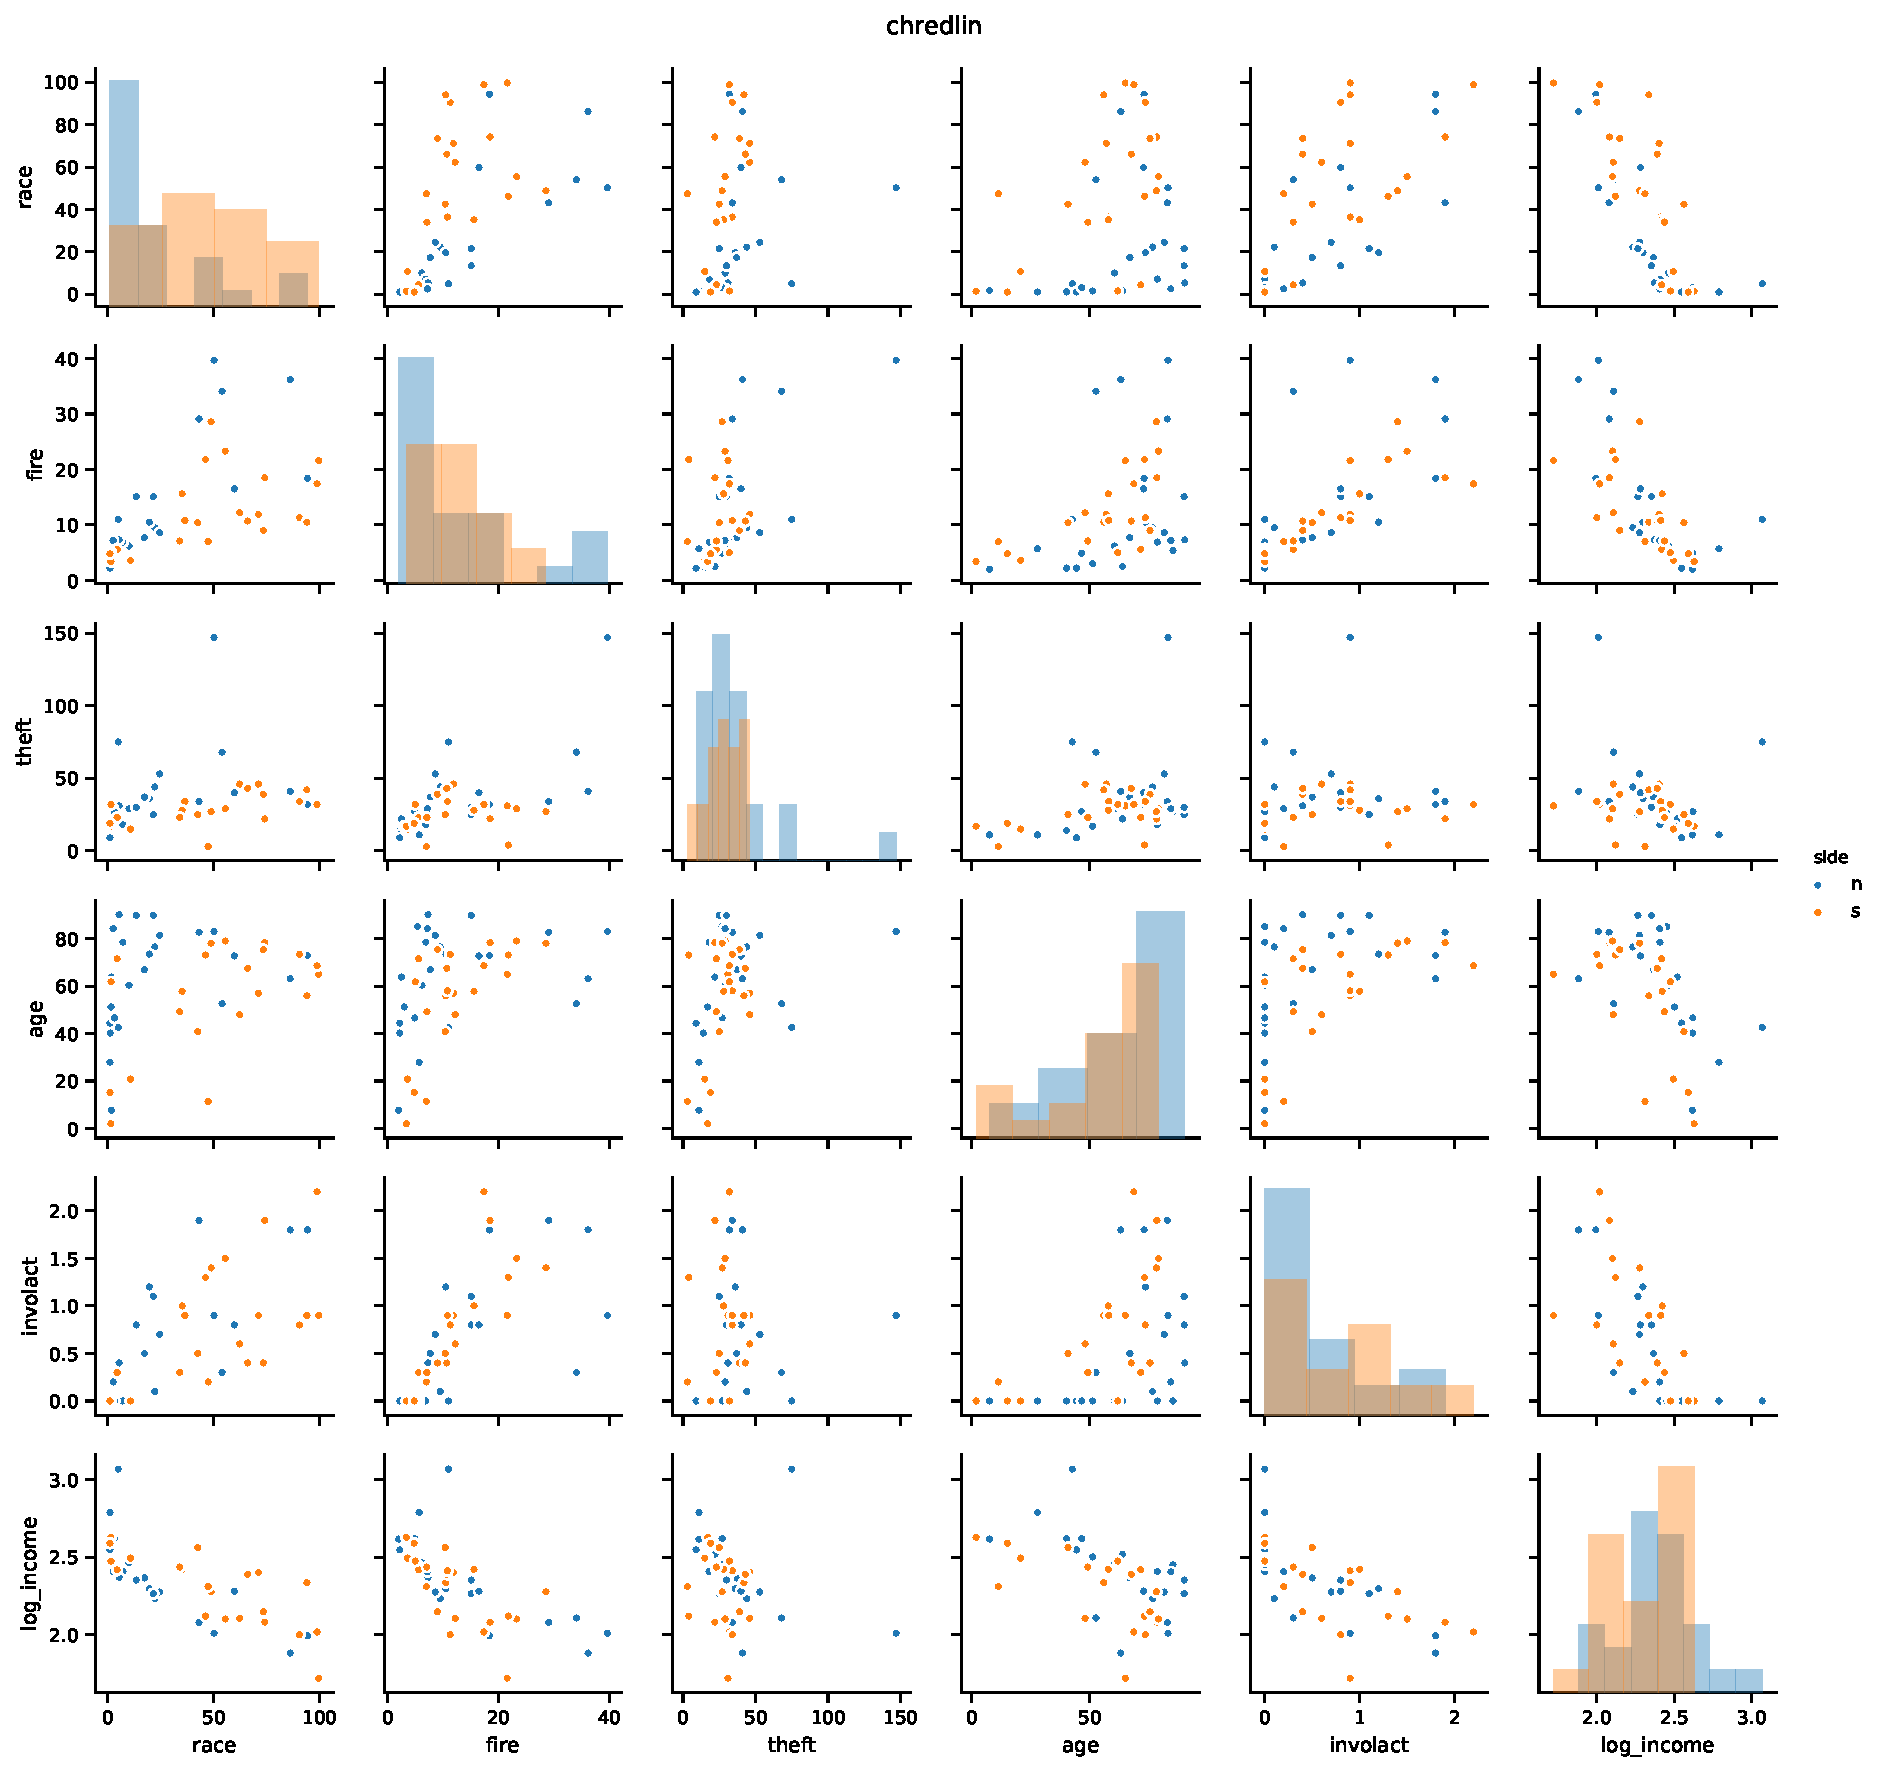
\includegraphics[width=\textwidth]{p1_pair_plots.pdf}
  \caption{The empirical univariate and joint distributions for the
    \texttt{chredlin} dataset.}
  \label{fig:p1_pair_plots}
\end{figure}

\end{document}

